\documentclass[a4paper,11pt]{article}
\usepackage[T1]{fontenc}
\usepackage[utf8]{inputenc}
\usepackage{graphicx}
\usepackage{xcolor}


\usepackage{amsmath,amssymb,amsthm,textcomp}
\usepackage{enumerate}
\usepackage{multicol}
\usepackage{tikz}
\usepackage[english, russian]{babel}

\usepackage{geometry}
\geometry{total={210mm,297mm},
	left=25mm,right=25mm,%
	bindingoffset=0mm, top=20mm,bottom=20mm}


% custom footers and headers
\usepackage{fancyhdr}
\pagestyle{fancy}
\rhead{\scriptsize ФКН НИУ ВШЭ, 2016/2017 учебный год, 1 курс ПМИ, Егерев Артем}
\lhead{\footnotesize Математический анализ}
\chead{}
\cfoot{}
\renewcommand{\headrulewidth}{0pt}
\renewcommand{\footrulewidth}{0pt}




%%%----------%%%----------%%%----------%%%----------%%%




\begin{document}
\textbf{\large Задача 1}
\medskip\hrule\medskip
\textit{Вычислите несобственные интегралы и установите их расходимость.(4)} \\ \\
Отметим, что наш несобстенный интеграл является интегралом первого рода, так как функция $ f(x) = \frac{(arctg x)^2}{1 + x^2} $ непрерывна на промежутке $ [\sqrt{3}, \infty) $. Согласно определению:
\begin{gather*}
\int\limits_{\sqrt{3}}^{+\infty} \frac{(arctg x)^2 dx}{1 + x^2} = 
\lim\limits_{b \to +\infty}\int\limits_{\sqrt{3}}^{b} \frac{(arctg x)^2 dx}{1 + x^2} =
\begin{vmatrix} t \equiv arctg x\end{vmatrix} = 
\lim\limits_{c \to \frac{\pi}{2}}\int\limits_{\frac{\pi}{3}}^{c} t^2dt = 
\Big|_{\frac{\pi}{3}}^{\frac{\pi}{2}} \; \frac{t^3}{3} = \frac{19\pi^3}{648} 
\end{gather*}
Получили константу, отсюда $ - $ интеграл сходится.
\\ \\ \\ 



\textbf{\large Задача 2}
\medskip\hrule\medskip
\textit{Исследуйте на сходимость несобственные интегралы.(8)} \\ \\
Сразу отметим, что наши несобстенные интеграл является интегралом первого рода, так интегрируемые функции непрерывны на заданных промежутах. Далее, согласно определению ищем предел:
\begin{enumerate}
	\item 
	$ 0 < \int\limits_{3}^{+\infty} \frac{(x^5 - x^2 + 4)dx}{3x^9 - 6x^4 + x + 7} = 
	\lim\limits_{b \to +\infty}\int\limits_{3}^{b} \frac{(x^5 - x^2 + 4)dx}{3x^9 - 6x^4 + x + 7} < 
	\lim\limits_{b \to +\infty}\int\limits_{3}^{b} \frac{x^5dx}{2x^9} = 
	\lim\limits_{b \to +\infty}\Big|_{3}^{b} (-\frac{1}{6x^3}) = \frac1{162} \\[4pt] \approx 0.0061728 \Rightarrow $  сходится
	
	\item
	$ \int\limits_{2}^{+\infty} \frac{\sqrt[3]{5x^2 + 2}dx}{x - 1} = 
	\begin{vmatrix} t \equiv x - 1 \end{vmatrix} =
	\int\limits_{1}^{+\infty} \frac{\sqrt[3]{5t^2 + 10t + 7}dx}{t} = 
	\int\limits_{1}^{+\infty} \sqrt[3]{\frac5{t} + \frac{10}{t^2} + \frac7{t^3}}dt = 
	\lim\limits_{b \to +\infty}\int\limits_{1}^{b} \sqrt[3]{\frac5{t} + \frac{10}{t^2} + \frac7{t^3}}dt >
	\lim\limits_{b \to +\infty}\int\limits_{1}^{b} \frac{dt}{t^{\frac13}} = 
	\lim\limits_{b \to +\infty}\Big|_{1}^{b} \frac32t^{\frac13} = \infty \Rightarrow
	$ расходится
	
	\item
	$ 0 < \int\limits_{1}^{+\infty} \frac{(x + 7 - cos 3x)dx}{x^3 + 5x^2 - 1} <	
	\int\limits_{1}^{+\infty} \frac{10xdx}{x^3} = 
	\lim\limits_{b \to +\infty} \int\limits_{1}^{b} \frac{10xdx}{x^3} = 
	\lim\limits_{b \to +\infty} \Big|_{1}^{b} (-\frac{10}{x}) = 10 \Rightarrow
	$ сходится
\end{enumerate}
.\\ \\ \\



\textbf{\large Задача 3}
\medskip\hrule\medskip
\textit{Вычислите несобственные интегралы и установите их расходимость.(12)}
\begin{gather*}
\int\limits_{-3}^{2} \frac{2x + 7}{\sqrt[3]{(x^2 + 7x + 12)^2}} = 
\begin{vmatrix} t \equiv x^2 + 7x + 12 \end{vmatrix} =
\int\limits_{0}^{30} \frac{dt}{t^{\frac23}} = 
\Big|_{0}^{30} 3t^{\frac13} = 3(30)^{\frac13} \approx 9.3217 \Rightarrow \text{сходится}
\end{gather*}
\newpage 



\textbf{\large Задача 4}
\medskip\hrule\medskip
\textit{Исследуйте на сходимость несобственные интегралы.(16)}
\begin{enumerate}
	\item 
	\begin{gather*}
	0 < \int\limits_{-1}^{2} \frac{\sqrt[4]{(x^2 + 3x + 2)^3}}{x^2 + 4x + 3}dx = 
	\int\limits_{-1}^{2} \sqrt[4]{\frac{(x + 2)^3}{(x + 1)(x + 3)^4}}dx < 
	\int\limits_{-1}^{2} \frac{dx}{(x + 1)^{\frac14}} = 
	\Big|_{-1}^{2} \frac43 (x + 1)^{\frac34} = \frac43 3^{\frac34} \\[2pt] \approx 3.0393 \Rightarrow \text{сходится}
	\end{gather*}
	
	\item Рассмотрим функцию $ g(x) =  \frac{x^2 / 2}{x\sqrt[3]{x}}:$
	\begin{gather*}
	\lim\limits_{x \to 0} \frac{f(x)}{g(x)} = 
	\lim\limits_{x \to 0} \frac{\sqrt{1 + x^2} - 1}{x^2/2} \cdot \frac{\sqrt[3]{x}}{e^{\sqrt[3]{x}} - 1} = 1 \neq 0 
	\end{gather*}
	В точке разрыва отношение функций есть константа, отсюда наши функции имеют одинаковый характер сходимости
	\begin{gather*}
	\int\limits_{0}^{5} g(x)dx =
	\int\limits_{0}^{5} \frac12 x^{\frac23}dx = 
	\Big|_{0}^{5} \frac3{10} x^{\frac53} = \frac3{2} 5^{\frac23} \approx 4.3860  \Rightarrow 
	\text{сходится}
	\end{gather*}
	
	\item Дейстуем аналогично 2 пункту, рассматриваем функцию $ g(x) =  \frac{x^{\frac32}}{x^3/3} $:
	\begin{gather*}
	\lim\limits_{x \to 0} \frac{f(x)}{g(x)} =
	\frac{x^3/3}{tg x - x} = 1 \neq 0
	\end{gather*}
	$ \int\limits_{0}^{3} g(x)dx =
	\int\limits_{0}^{3} 3 \frac1{x^{\frac32}}dx = 
	\Big|_{0}^{3} (-\frac32) \frac1{x^{\frac12}} = \infty \Rightarrow 
	$ расходится
\end{enumerate}
.
\\ \\ \\




\textbf{\large Задача 5}
\medskip\hrule\medskip
\textit{Найдите все значения параметра $ \alpha $, при которых сходится интеграл.(20)}
\begin{enumerate}
	\item  \begin{gather*}
	\int\limits_{-1}^{4} \frac{log_2^{\alpha}(x + 2)}{(1 + x^5)^{\alpha^2}}dt = 
	\begin{vmatrix} t \equiv arctg x + 1 \end{vmatrix} = 
	\int\limits_{0}^{5} \frac{log_2^{\alpha}(1 + t)}{(t^5 - 5 t^4 + 10 t^3 - 10 t^2 + 5 t)^{\alpha^2}}dt 
	\end{gather*}
	Разрыв в 0, где по ряду Тейлора можем заменить на эквивалентный по сходимости интеграл:
	\begin{gather*}
	\int\limits_{0}^{5} \frac{t^{\alpha}}{t^{\alpha^2}}dt
	\end{gather*}
	Для того, чтобы интеграл сходился, требуется $ \alpha^2 - \alpha < 1 \Rightarrow \alpha^2 - \alpha - 1 < 0 \Rightarrow \alpha \in (0, 1) $. В остальных случаях расходится.
	
	
	\item Здесь неопределенность возникает уже на бесконечности.  Аналогично, заменяем на бесконечности:
	\begin{gather*}
	\Big(\frac{5x - 1}{3x + 1}\Big)^{\alpha x} (ln(2 + 3^{\alpha^2x}) - ln(1 + 3^{\alpha^2x})) \equiv e^{\alpha x}  (ln(1 + \frac2{3^{\alpha^2x}}) - ln(1 + \frac1{3^{\alpha^2x}})) \equiv \\[2pt] \equiv
	\frac{e^{\alpha x}}{e^{\alpha^2 x}}
	\end{gather*}
	Сходится, когда $ \alpha < \alpha^2 \Rightarrow \alpha \in (-\infty, 0) \cup (1, \infty) $ 
\end{enumerate}
\newpage






\textbf{\large Задача 6}
\medskip\hrule\medskip
\textit{Исследуйте несобственный интеграл на абсолютную и условную сходимость.(24)} \\ \\
Сделаем замену переменных $ t \equiv \sqrt{x + 1} - 1 $. $ dx = d((t + 1)^2 - 1) = 2(t + 1)dt $
\begin{gather*}
\int\limits_{\sqrt{2} - 1}^{\infty} \frac{2cos(t) \cdot (t + 1)}{(t + 1)^2 - 1 + sin((t + 1)^2 - 1)}dt
\end{gather*}
По аналогии с предыдущими рассуждениями данный интеграл эквивалентен:
\begin{gather*}
\int\limits_{\sqrt{2} - 1}^{\infty} \frac{cos(t)}{t}dt - \text{сходится}
\end{gather*}
Докажем абсолютню расходимость:
\begin{gather*}
\int\limits_{\sqrt{2} - 1}^{\infty} \Big|\frac{cos(t)}{t}\Big|dt = 
\int\limits_{\sqrt{2} - 1}^{\infty} \frac{|cos(t)|}{t}dt - \text{расходится}
\end{gather*}
Таким образом, интеграл условно сходится.
\\ \\ \\





\textbf{\large Задача 7}
\medskip\hrule\medskip
\textit{Найлите аналитически (в явном виде или параметрически) границы клеток Вороного для точечных множеств $ M $ в $ \mathbb{R}^n $(28):}
\begin{itemize}
	\item \textit{в пукте а для метрик $ d_1 = \sum_{i = 1}^{n}|x_i - y_i|, d_2 = \sqrt{\sum_{i = 1}^{n}|x_i - y_i|^2}, d_{\infty} = max|x_i - y_i| $}
	
	\item \textit{в пункте б для метрики $ d_2 $. В пункте а постойте все границы.}
\end{itemize}  
\begin{enumerate}
	\item $ x_1(1, -3), \; x_2(-4, 2) $. Аналитически уравнение будет выглядить следующим образом:
	\begin{enumerate}
		\item $ |1 - x| + |-3 - y| = |-4 - x| + |2 - y| $ для $ d_1 $ 
		\item $ \sqrt{(1 - x)^2 + (-3 - y)^2} = \sqrt{(-4 - x)^2 + (2 - y)^2} $ для $ d_2 $
		\item $ max(1 - x, -3 - y) = max(-4 - x, 2 - y) $ для $ d_{\infty} $
	\end{enumerate}
	Где $ (x, y) - $ искомая клетка Вороного. Выполним переход от уравнения к системе:
	\begin{enumerate}
		\item 
		$\left[\begin{array}{l}
		x \leqslant -4, y \leqslant -3 \\[2pt]
		-4 < x < 1, \; y = x + 1 \\[2pt]
		x \geqslant 1, y \geqslant 2
		\end{array}\right.$
		\begin{center}
			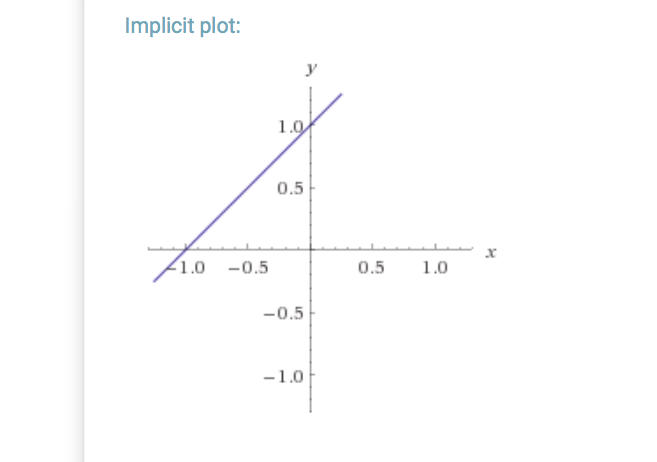
\includegraphics[width = 60mm, height=40mm]{images/1.png}
		\end{center}
		
		\item 
		$\left[\begin{array}{l}
		y = x  +1
		\end{array}\right.$
		\begin{center}
			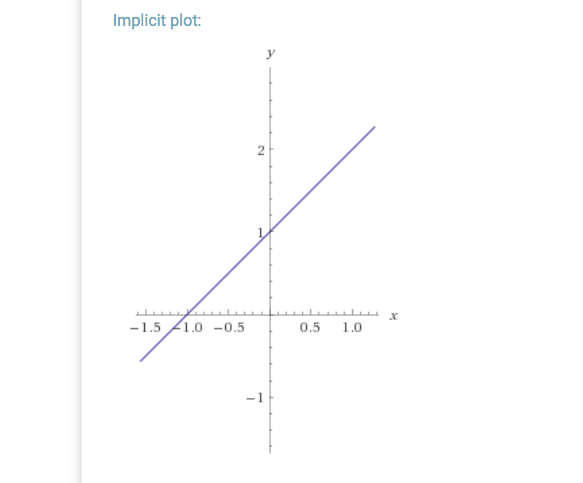
\includegraphics[width = 60mm, height=40mm]{images/2.png}
		\end{center}
		
		\item 
		$\left[\begin{array}{l}
		y = x  +1
		\end{array}\right.$
		\begin{center}
			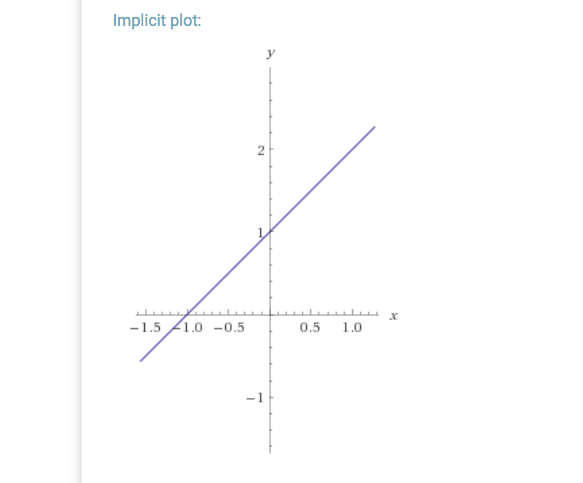
\includegraphics[width = 60mm, height=40mm]{images/2.png}
		\end{center}
	\end{enumerate}
	
	\item $ x_1(3, 2, -4), \; x_2(2, 1, 5) $ \\[6pt]
	$ \sqrt{(3 - x)^2 + (2 - y)^2 + (-4 - z)^2} = \sqrt{(2 - x)^2 + (1 - y)^2 + (5 - z)^2} $ \\[6pt] 
	Откуда имеем: $ z = \frac1{18}(2x + 2y + 1) $
\end{enumerate}
. \\ \\ \\






\textbf{\large Задача 8}
\medskip\hrule\medskip
\begin{itemize}
	\item \textit{найдите линии уровня $ f(x, y) = C $, определите тип (второго порядка) в зависимости от значения $ C $, найдите их ось симметрии, постройте по одной кривой различных типов.(2)}
	
	\item  \textit{найдите пределы $ \lim\limits_{x \to x_1 \; y \to y_1} f(x, y) $ и $ \lim\limits_{x \to x_2 \; y \to y_2} f(x, y) $}
\end{itemize}



\begin{enumerate}
	\item $ \dfrac{3x^2 - xy}{x^2 - y^2}, \; (x_1, y_1) = (-2, 1), \; (x_2, y_2) = (0, 0), \text{ Одз } x \neq \pm y $ \\[6pt]
	\begin{gather*}
	f(x, y) = C = \dfrac{3x^2 - xy}{x^2 - y^2} \Rightarrow Cy^2 - xy + 3x^2 - Cx^2 = 0 \Rightarrow \\[2pt]
	x = y\dfrac{1 \pm \sqrt{1 - 4c(3 - c)}}{2(3 - c)} = 
	y\dfrac{1 \pm \sqrt{4(c - \frac32 - \sqrt{2})(c - \frac32 + \sqrt{2}))}}{2(3 - c)}
	\end{gather*}
	Отсюда вытекает несколько случае:
	\begin{enumerate}
		\item $ C = 3 $ \\[2pt]
		$ 3y^2 - xy + 3x^2 - 3x^2 = (3y - x)y = 0 $ - две прямые 
		$ y = tg(\frac{\alpha}2)x  =  (\sqrt{10} - 3)x $, где $ tg(\alpha) = \frac13 $ - ось симметрии \\
		$ (0, 0) - $ выколотая
		\begin{center}
			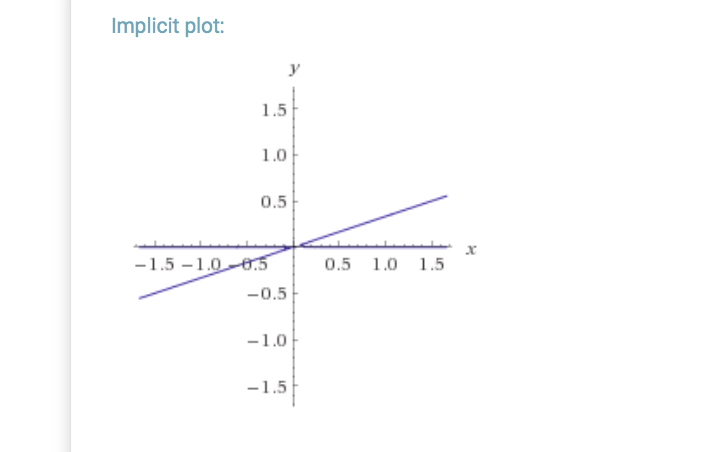
\includegraphics[width = 60mm, height=40mm]{images/3.png}
		\end{center}
		
		
		\item $ C = \frac32 \pm \sqrt{2} $ \\ 
		Вырожденные случаи, $ y = \frac{1}{2(3 - c)} - $ одна прямая, она же ось симметрии \\
		$ (\frac{1}{2(3 - c)}, \frac{1}{2(3 - c)}) - $ выколотая
		\begin{center}
			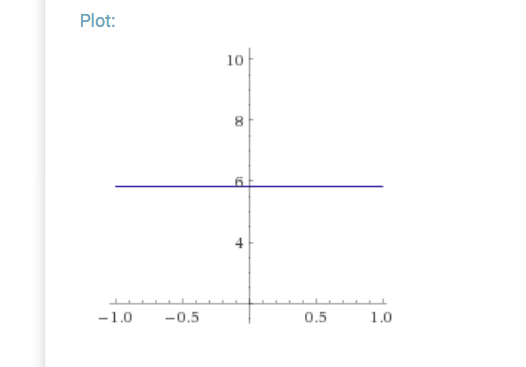
\includegraphics[width = 60mm, height=40mm]{images/4.png}
		\end{center}
		
		
		\item $ C \in (\frac32 - \sqrt{2}, \frac32 + \sqrt{2}) $ - решений нет
		
		
		
		\item в остальных случаях получаем две прямые $ x = y\dfrac{1 \pm \sqrt{4(c - \frac32 - \sqrt{2})(c - \frac32 + \sqrt{2}))}}{2(3 - c)} $ \\
		ось симметрии $ - $ полусумма $ x_i $ при одном $ y \Rightarrow  x = y\frac{1}{3 - c}$   
		\begin{center}
			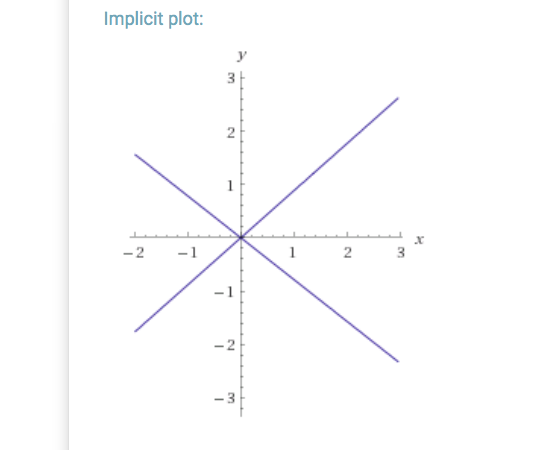
\includegraphics[width = 60mm, height=40mm]{images/5.png}
		\end{center}
	\end{enumerate}
	.\\
	
	
	
	
	\item 
	\begin{itemize}
		\item $ \lim\limits_{x \to x_1 \; y \to y_1} f(x, y) = 
		\lim\limits_{x \to -2 \; y \to 1} \dfrac{3x^2 - xy}{x^2 - y^2} =
		\dfrac{3\cdot4 + 2 \cdot 1}{4 - 1} = \dfrac{14}3
		$
		
		\item $ \lim\limits_{x \to x_2 \; y \to y_2} f(x, y) = 
		\lim\limits_{x \to 0 \; y \to 0} \dfrac{3x^2 - xy}{x^2 - y^2} =
		\dfrac{3cos^2\alpha - 2sin\alpha \cdot cos\alpha}{cos^2\alpha - sin^2\alpha} =
		\dfrac{3 - 2tg\alpha}{1 - tg^2\alpha} - \\[5pt]
		$ зависит от $ \alpha $, поэтому предела не существует.
	\end{itemize}
\end{enumerate}
\newpage


\textbf{\large Задача 9}
\medskip\hrule\medskip
\textit{Найдите $ \frac{\partial u}{\partial x}, \frac{\partial u}{\partial y}, \frac{\partial u}{\partial z} $ для функции $ u = f(x, y, z) $ и значение частной производной в указанной точке.(6)} \\ \\ \\
$ f(x, y, z) = y^2sin(xyz) $
\begin{enumerate}
	\item $ \frac{\partial u}{\partial x} = y^3 \cdot z \cdot cos(xyz) $
	\item $ \frac{\partial u}{\partial y} = y(2sin(xyz) + xyz \cdot cos(xyz)) $
	\item $ \frac{\partial u}{\partial z} = y^3 \cdot x \cdot cos(xyz) $
\end{enumerate}
$ u_{y}^{'}(0, 21, -1) = 0 $
\\ 



\textbf{\large Задача 10}
\medskip\hrule\medskip
\textit{Найдите все частные производные второго порядка функции $ u = f(x, y, z) $. Найдите значение указанной частной производной в заданной точке.(10)} \\ \\
$ f(x, y, z) = 2x^3y^2 - y^2z^2 + xz^3 $
\begin{enumerate}
	\item 
	$ \frac{\partial u}{\partial x} = 4x^2y^2 + z^3 $
	\begin{enumerate}
		\item $ \frac{\partial}{\partial x}(\frac{\partial u}{\partial x}) = 8xy^2 $
		\item $ \frac{\partial}{\partial y}(\frac{\partial u}{\partial x}) = 8x^2y $
		\item $ \frac{\partial}{\partial z}(\frac{\partial u}{\partial x}) = 3z^2 $
	\end{enumerate}
	
	\item
	$ \frac{\partial u}{\partial y} = 4x^3y - 2yz^2 $
	\begin{enumerate}
		\item $ \frac{\partial}{\partial x}(\frac{\partial u}{\partial y}) = 12x^2y $ 
		\item $ \frac{\partial}{\partial y}(\frac{\partial u}{\partial y}) = 4x^3 - 2z^2 $
		\item $ \frac{\partial}{\partial z}(\frac{\partial u}{\partial y}) = -4yz $
	\end{enumerate}
	
	\item
	$ \frac{\partial u}{\partial z} = -2y^2z + 3xz^2 $
	\begin{enumerate}
		\item $ \frac{\partial}{\partial x}(\frac{\partial u}{\partial z}) = 3z^2 $
		\item $ \frac{\partial}{\partial y}(\frac{\partial u}{\partial z}) = -4yz $
		\item $ \frac{\partial}{\partial z}(\frac{\partial u}{\partial z}) = -2y^2 + 6xz $
	\end{enumerate}
\end{enumerate}
$ u''_{yz}(1, 2, 1) = -8 $
\\ 


\textbf{\large Задача 11}
\medskip\hrule\medskip
\textit{Докажите, что функция $ z = f(x, y) $  удволетворяет дифференциальному уравнению в частных производных $ F(\dots) = 0 $.(14)} \\ \\ 
$ z = arctg \frac{x + y}{1 - xy} \quad F = \frac{\partial^2 z}{\partial x \partial y}$
\begin{enumerate}
	\item $ \frac{\partial z}{\partial x} = \frac1{1 + (\frac{x + y}{1 - xy})^2}  \cdot 
	\frac{(1 - xy) + y(x + y)}{(1 - xy)^2} = \frac{1}{x^2 + 1} $
	
	\item $ \frac{\partial}{\partial y}(\frac{\partial z}{\partial x}) = 0 $
\end{enumerate}
Действительно :)
\newpage






\textbf{\large Задача 12}
\medskip\hrule\medskip
\textit{Найдите $ du $ и $ d^2u $ для функции $ u = f(x, y) $.(18)} \\ \\
$ u = -x^4y^4 + 3x^2 $
\begin{enumerate}
	\item $ \frac{\partial u}{\partial x} = -4x^3y^4 + 6x $
	\begin{enumerate}
		\item $ \frac{\partial }{\partial x} (\frac{\partial u}{\partial x}) = -12x^2y^4 + 6 $
		
		\item $ \frac{\partial }{\partial x} (\frac{\partial u}{\partial y}) = -16x^3y^3 $
	\end{enumerate}
	
	\item $ \frac{\partial u}{\partial y} = -4x^4y^3 $
	\begin{enumerate}
		\item $ \frac{\partial }{\partial x} (\frac{\partial u}{\partial y}) = -16x^3y^3 $
		
		\item $ \frac{\partial }{\partial y} (\frac{\partial u}{\partial y}) = -12x^4y^2 $
	\end{enumerate}
\end{enumerate}
Теперь, когда уже все знаем, мы готовы выписать ответ:
\begin{enumerate}
	\item $ du = \frac{\partial u}{\partial x}dx + \frac{\partial u}{\partial y}dy = 
	(-4x^3y^4 + 6x)dx - 4x^4y^3dy
	$
	
	\item $ d^2 u = \frac{\partial^2 u}{\partial x \partial x} dx^2 + 
	\frac{\partial^2 u}{\partial x \partial y} dx dy + 
	\frac{\partial^2 u}{\partial y \partial x} dx dy +
	\frac{\partial^2 u}{\partial y \partial y} dy^2 = \\[4pt] = 
	(-12x^2y^4 + 6)\cdot dx^2 - 16x^3y^3 \cdot dxdy - 16x^3y^3 \cdot dxdy - 12x^4y^2 \cdot dy^2 = \\[4pt] = 
	(-12x^2y^4 + 6)\cdot dx^2 - 32x^3y^3 \cdot dxdy - 12x^4y^2 \cdot dy^2 
	$
\end{enumerate}
. \\ \\ \\






\textbf{\large Задача 13}
\medskip\hrule\medskip
\begin{itemize}
	\item \textit{составьте уравнение касательной плоскости и нормали к поверхности, заданной уравнением $ f(x, y, z) = 0 $, в указанной точке $ M $}
	
	\item \textit{найдите наибольшую скорость возрастания функции  $ f(x, y, z) = 0 $ в точке $ M $}
	
	\item \textit{найдите производнуб функции $ f(x, y, z) $ в точке $ M $ по направлению вектора $ l $ \quad (22)}
\end{itemize} 
\begin{enumerate}
	\item $ f(x, y, z) = 3x^2 + 4xy^2z - 2yz^2 - y^3 - 6z^3 - 12, \; M(2, 1, 1) $ \\[4pt]
	Ищем все частные производные:
	\begin{enumerate}
		\item $
		\frac{\partial f}{\partial x} = 6x + 4y^2z =  16
		$
		
		\item $
		\frac{\partial f}{\partial y} = 8xyz - 2z^2 - 3y^2 =  11 
		$
		
		\item $
		\frac{\partial f}{\partial z} = 4xy^2 - 4yz - 18z^2  = -14 
		$
	\end{enumerate}
	Отсюда 
	\begin{enumerate}
		\item $ \dfrac{\partial z}{\partial x} = -\dfrac{\frac{\partial f}{\partial x}}{\frac{\partial f}{\partial z}} = -\dfrac{6x + 4y^2z}{4xy^2 - 4yz - 18z^2} = -\dfrac{3x + 2y^2z}{2xy^2 - 2yz - 9z^2} $
		
		\item $ \dfrac{\partial z}{\partial y} = -\dfrac{\frac{\partial f}{\partial y}}{\frac{\partial f}{\partial z}} = -\dfrac{8xyz - 2z^2 - 3y^2 }{4xy^2 - 4yz - 18z^2} $
	\end{enumerate}
	$ z - z_0 = z'_x(x_0, y_0, z_0)(x - x_0) + z'_y(x_0, y_0, z_0)(y - y_0)  \; - $ уравнение касательной
	\begin{enumerate}
		\item $ z'_x(2, 1, 1) =  \frac87 $
		
		\item $ z'_y(2, 1, 1) =  \frac{11}{14} $
		
	\end{enumerate}
	$ z - 1 = \frac87(x - 1) + \frac{11}{14}(y - 1) \Rightarrow -\frac{8x}{7} - \frac{11y}{14} + z + \frac{13}{14} = 0 $ \\[2pt]
	$ \dfrac{x - x_0}{z'_x} = \dfrac{y - y_0}{z'_y} = \dfrac{z - z_0}{-1} $ - нормаль \\[4pt]
	$ \dfrac{x - 2}{(\frac87)} =  \dfrac{y - 1}{(\frac{11}{14})} = -(z - 1) $ - формула нормали к поверхности в заданной точке
	
	
	\item $ grad(f) = \frac{\partial f}{\partial x} \vec{i} + \frac{\partial f}{\partial y} \vec{j} + \frac{\partial f}{\partial z} \vec{k} = 16\vec{i} + 11\vec{j} - 14\vec{k} $ \\[2pt]
	$ |grad(f)| = \sqrt{(16)^2 + (11)^2 + (14)^2} = \sqrt{573} $ - наибольшая скорость возрастания функции
	
	\item
	$
	\frac{\partial f}{\partial l} = \frac{\partial f}{\partial x} cos(\alpha) + \frac{\partial f}{\partial y} cos(\beta) + \frac{\partial f}{\partial z} cos(\gamma)  
	$, где $ cos(\alpha) = \frac{-1}{\sqrt{6}}, \;  cos(\beta) = \frac{1}{\sqrt{6}}, \;  cos(\gamma) = \frac2{\sqrt{6}} $ \\[4pt]
	$ \frac{\partial f}{\partial l} = \frac{-16}{\sqrt{6}} + \frac{11}{\sqrt{6}} - \frac{14 \cdot 2}{\sqrt{6}} = -\frac{11\sqrt{6}}{2}$
\end{enumerate}
.
\\ \\ \\




\textbf{\large Задача 14}
\medskip\hrule\medskip
\textit{Пользуясь правилом дифференцирования сложной функции, найдите $ \frac{\partial u}{\partial t}, \; \frac{\partial u}{\partial v} $ для заданных функций $ u = u(x, y), \; x = x(t, v), \; y = y(t, v) $.(26)} \\ \\
$ u = x^3cos(5x - 3y) \quad x = t \cdot arcsin(t^2v) \quad y = e^{t - v^2} $
\begin{enumerate}
	\item $ \frac{\partial u}{\partial x} = 
	x^2(3cos(5x - 3y) - 5x\cdot sin(5x - 3y))
	$
	
	\item $ \frac{\partial u}{\partial y} = 
	3x^3\cdot sin(5x - 3y)
	$
	
	\item $ 
	\frac{\partial x}{\partial t} = 
	arcsin(t^2v) + \frac{2t^2}{\sqrt{1 - (t^2v)^2}}
	$
	
	\item $ 
	\frac{\partial x}{\partial v} = 
	\frac{t}{\sqrt{1 - (t^2v)^2}}
	$
	
	\item $ 
	\frac{\partial y}{\partial t} = 
	e^{t - v^2}
	$
	
	\item $ 
	\frac{\partial y}{\partial v} = 
	-2ve^{t - v^2} 
	$
\end{enumerate}
Все знаем, пишем формулу:
\begin{enumerate}
	\item $ \frac{\partial u}{\partial t} = \frac{\partial u}{\partial x} \cdot \frac{\partial x}{\partial t} + 
	\frac{\partial u}{\partial y} \cdot \frac{\partial y}{\partial t} = 
	x^2(3cos(5x - 3y) - 5x\cdot sin(5x - 3y))(arcsin(t^2v) + \frac{2t^2}{\sqrt{1 - (t^2v)^2}}) + \\[2pt] + \;  
	3x^3\cdot sin(5x - 3y)e^{t - v^2}
	$
	
	\item $ \frac{\partial u}{\partial v} = \frac{\partial u}{\partial x} \cdot \frac{\partial x}{\partial v} + 
	\frac{\partial u}{\partial y} \cdot \frac{\partial y}{\partial v} = 
	x^2(3cos(5x - 3y) - 5x\cdot sin(5x - 3y))\frac{t}{\sqrt{1 - (t^2v)^2}} \; - \;   
	6x^3\cdot sin(5x - 3y)ve^{t - v^2}
	$
	
\end{enumerate}
.
\\ \\ 



\textbf{\large Задача 15}
\medskip\hrule\medskip
\textit{Найдите $ y'_x $ для функции, заданной неявно.(30)}
\begin{gather*}
y^2arctg(2x) - xtg(2x + 3y) = 0 \text{ | берем производную по $ x $ от левой и правой части} \\[2pt]
2yy'_x \cdot arctg(2x) + \frac{2y^2}{1 + 4x^2} - tg(2x + 3y) - \frac{2x}{cos^2(2x + 3y)} = 0 \\[2pt]
y'_x = \frac{tg(2x + 3y) + \frac{2x}{cos^2(2x + 3y)} - \frac{2y^2}{1 + 4x^2}}{2y \cdot arctg(2x)}
\end{gather*}
\newpage



\textbf{\large Задача 16}
\medskip\hrule\medskip
\textit{Найдите $ \frac{\partial z}{\partial x}, \frac{\partial z}{\partial y} $ для функции $ z = z(x, y) $, заданной неявно указанным уравнением.(4)} \\ \\
$ F = (y - 3z)^2 - 5sin(x + 2z) = 0 $
\begin{enumerate}
	\item $
	\frac{\partial F}{\partial x} = -5cos(x + 2z) 
	$
	
	\item $
	\frac{\partial F}{\partial y} = 2(y - 3z) = 2y - 6z 
	$
	
	\item $
	\frac{\partial F}{\partial z} = -6(y - 3z) + 10cos(x + 2z)
	$
\end{enumerate}
Отсюда, снова легко находим частные производные:
\begin{enumerate}
	\item $ \dfrac{\partial z}{\partial x}  = -\dfrac{\frac{\partial F}{\partial x}}{\frac{\partial F}{\partial z}} = -\dfrac{-5cos(x + 2z)}{-6(y - 3z) + 10cos(x + 2z)} = \dfrac{5cos(x + 2z)}{10cos(x + 2z) - 6(y - 3z)} $
	
	\item $ 
	\dfrac{\partial z}{\partial y}  = -\dfrac{\frac{\partial F}{\partial y}}{\frac{\partial F}{\partial z}} = -\dfrac{2y - 6z}{-6(y - 3z) + 10cos(x + 2z)} = \dfrac{2y - 6z}{6(y - 3z) - 10cos(x + 2z)}
	$
\end{enumerate}
.\\ \\ \\



\textbf{\large Задача 17}
\medskip\hrule\medskip
\textit{Найдите разложение функции $ u(x, y) $ по формуле Маклорена до $ o((x^2 + y^2)^{\frac{n}2}) $.(8)}
\begin{gather*}
u(x, y) = \frac{1}{\sqrt[4]{16 + 4x^2 + 8y^2}} = \frac1{2\sqrt[4]{1 + \frac{x^2}{4} + \frac{y^2}{2}}} = \frac1{2\sqrt[4]{1 + t}} = \frac12(1 + t)^{-\frac14}, \text{ где $ t \equiv \frac{x^2}{4} + \frac{y^2}{2} $ } \\[4pt]
u(t) = \frac12(1 + \sum\limits_{n = 1}^{\infty} \begin{pmatrix} \alpha \\ n \end{pmatrix}t^{n}) =  \frac12(1 + \sum\limits_{n = 1}^{\infty} \begin{pmatrix} \alpha \\ n \end{pmatrix}\big(\frac{x^2}{4} + \frac{y^2}{2}\big)^{n} + o((x^2 + y^2)^{\frac{n}2})
\end{gather*}
\\ \\ \\



\textbf{\large Задача 18}
\medskip\hrule\medskip
\textit{Найдите разложение по формуле Тейлора до второго порядка.(12)}
\begin{gather*}
u(x, y, z) = sin^2(\frac{\pi}4(2x + z))cos(\frac{\pi}6y) \qquad (x_0, y_0, z_0) = (-1, 2, 2)
\end{gather*}
\begin{enumerate}
	\item $
	\frac{\partial u}{\partial x} = \frac12\pi cos(\frac{\pi y}{6})sin(\frac12 \pi (2x + z))) = 0  
	$
	
	\item $
	\frac{\partial u}{\partial y} = -\frac16 \pi sin(\frac{\pi y}{6}) sin^2(\frac14  \pi (2x + z))) = 0  
	$
	
	\item $
	\frac{\partial u}{\partial z} = \frac14\pi cos(\frac{\pi y}{6})sin(\frac12 \pi (2x + z)))   = 0  
	$
	
	\item $ \frac{\partial^2 u}{\partial x \partial x} = \frac12 \pi^2 cos(\frac{\pi y}{6}) cos(\frac12 \pi (2x + z)) = \frac{\pi^2}{4}	
	$
	
	\item $ \frac{\partial^2 u}{\partial x \partial y} = -\frac1{12} \pi^2 sin(\frac{\pi y}{6}) sin(\frac12 \pi (2x + z)) = 0
	$
	
	\item $ \frac{\partial^2 u}{\partial x \partial z} = \frac14 \pi^2 cos(\frac{\pi y}{6}) cos(\frac12 \pi (2x + z)) = \frac{\pi^2}{8}
	$
	
	\item $ \frac{\partial^2 u}{\partial y \partial x} = -\frac1{12} \pi^2 sin(\frac{\pi y}{6}) sin(\frac12 \pi (2x + z)) = 0
	$
	
	\item $ \frac{\partial^2 u}{\partial y \partial y} = -\frac1{36} \pi^2 cos(\frac{\pi y}{6}) sin^2(\frac14 \pi (2x + z)) = 0
	$
	
	\item $ \frac{\partial^2 u}{\partial y \partial z} = -\frac1{24} \pi^2 sin(\frac{\pi y}{6}) sin(\frac14 \pi (2x + z)) = 0
	$
	
	\item $ \frac{\partial^2 u}{\partial z \partial x} = \frac1{4} \pi^2 cos(\frac{\pi y}{6}) cos(\frac14 \pi (2x + z)) = \frac{\pi^2}{8}
	$
	
	\item $ \frac{\partial^2 u}{\partial z \partial y} = -\frac1{24} \pi^2 sin(\frac{\pi y}{6}) sin(\frac14 \pi (2x + z)) = 0
	$
	
	\item $ \frac{\partial^2 u}{\partial z \partial z} = -\frac1{24} \pi^2 sin(\frac{\pi y}{6}) sin(\frac14 \pi (2x + z)) = \frac{\pi^2}{16}
	$
\end{enumerate}
\begin{gather*}
u(x, y, z) = u_0(x, y, z) + u'\delta + \frac{u''\delta^2}{2!} + o(\delta^2) = 
(0 + 0 + 0)\delta + (\frac{\pi^2}{4} + \frac{\pi^2}{8} + \frac{\pi^2}{8} + \frac{\pi^2}{16})\delta^2 + o(\delta^2) = \frac{9\pi^2\delta^2}{16} + o(\delta^2)
\end{gather*}
где $ \delta = \sqrt{(x - x_0)^2 + (y - y_0)^2 + (z - z_0)^2} $
\\ \\ \\





\textbf{\large Задача 20}
\medskip\hrule\medskip
\textit{Найти частные производные и точные значения функций.(20) }
\begin{gather*}
\begin{cases}
2u^2v - v^2 + x^2y - y = 0 \\[2pt]
u^2 - v - 3x + 4y = 0
\end{cases}
\end{gather*}
Дифференцируя по $ x $ и $ y $ получаем систему из 4 уравнений:
\begin{gather*}
\begin{cases}
4uu'_xv + 2u^2v'_x - 2vv'_x + 2xy = 0 \\[2pt]
2uu'_x - v'_x - 3 = 0 \\[2pt]
4uu'_yv + 2u^2v'_y - 2vv'_y + x^2 - 1 = 0 \\[2pt]
2uu'_y - v'_y + 4 = 0
\end{cases}
\begin{cases}
4uvu'_x + 2(u^2  - v)v'_x  = -2xy\\[2pt]
2uu'_x - v'_x = 3 \\[2pt]
4uvu'_y + 2(u^2 - v)v'_y = 1 - x^2 \\[2pt]
2uu'_y - v'_y = -4
\end{cases}
\end{gather*}
\begin{gather*}
\sigma = -4uv - 4u(u^2 - v) = -4u^3 \\[2pt]
\sigma_x = -2xy(-1) - 6(u^2 - v) = 2xy - 6(u^2 - v) \\[2pt] 
\sigma_y = 12uv  + 4xyu  \\[2pt]
u'_x = \frac{2xy - 6(u^2 - v)}{-4u^3} \quad v'_x = -\frac{3v  + xy}{u^2}
\\ \\
\sigma = -4uv - 4u(u^2 - v) = -4u^3 \\[2pt]
\sigma_x = (1 - x^2)(-1) + 8 = x^2 + 7 \\[2pt]
\sigma_y = -16uv  - 2u(1 - x^2) = -2u(1 - x^2 + 16v) \\[2pt]
u'_y = -\frac{x^2 + 7}{4u^3} \quad u'_y = \frac{1 - x^2 + 16v}{2u^2} 
\end{gather*}
Подставляем нашу точку и находим значения функций:
\begin{gather*}
\begin{cases}
2u^2v - v^2 - 6 = 0 \\[2pt]
u - v - 14 = 0
\end{cases}
\end{gather*}
\begin{center}
	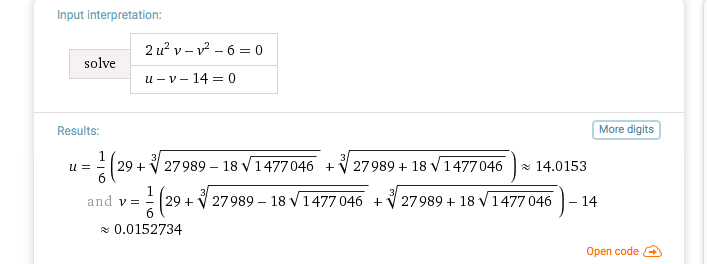
\includegraphics[width = 100mm, height=40mm]{images/6.png}
\end{center}
\newpage 




\textbf{\large Задача 21}
	\medskip\hrule\medskip
	\textit{Найдите и изобразите $ D $ и $ G $.(24)}
	\begin{gather*}
	\begin{cases}
	-1 \leqslant y \leqslant 1 \\[2pt]
	1 \leqslant 2y - 3x \leqslant 4 
	\end{cases}
	\begin{cases}
	x = -u + 4v \\[2pt]
	y = u + 2v
	\end{cases}
	\end{gather*}
	
	\begin{gather*}	
	\begin{cases}
	-1 \leqslant -u + 4v \leqslant 1 \\[2pt]
	1 \leqslant 5u - 8v \leqslant 4
	\end{cases}	
	\Rightarrow
	\begin{cases}
	-5 \leqslant -5u + 20v \leqslant 5 \\[2pt]
	1 \leqslant 5u - 8v \leqslant 4
	\end{cases}
	\Rightarrow	
	\begin{cases}
	-4 \leqslant 12v \leqslant 9
	\end{cases}
	\\[2pt]	
	\Rightarrow
	\begin{cases}
	-\frac13 \leqslant v \leqslant \frac34 \\[2pt]
	\end{cases}
	\Rightarrow
	\begin{cases}
	1 + 8v \leqslant 5u \leqslant 4 + 8v \\[2pt]
	\end{cases}
	\end{gather*}
	\begin{gather*}
	\begin{cases}
	-1 \leqslant y \leqslant 1 \\[2pt]
	-4 + 2y \leqslant 3x \leqslant -1 + 2y 
	\end{cases}
	\end{gather*}
	Теперь строим:
	\begin{gather*}
	\begin{cases}
	-\frac13 \leqslant v \leqslant \frac34 \\[2pt]
	1 + 8v \leqslant 5u \leqslant 4 + 8v
	\end{cases}
	\end{gather*}
	\begin{center}
		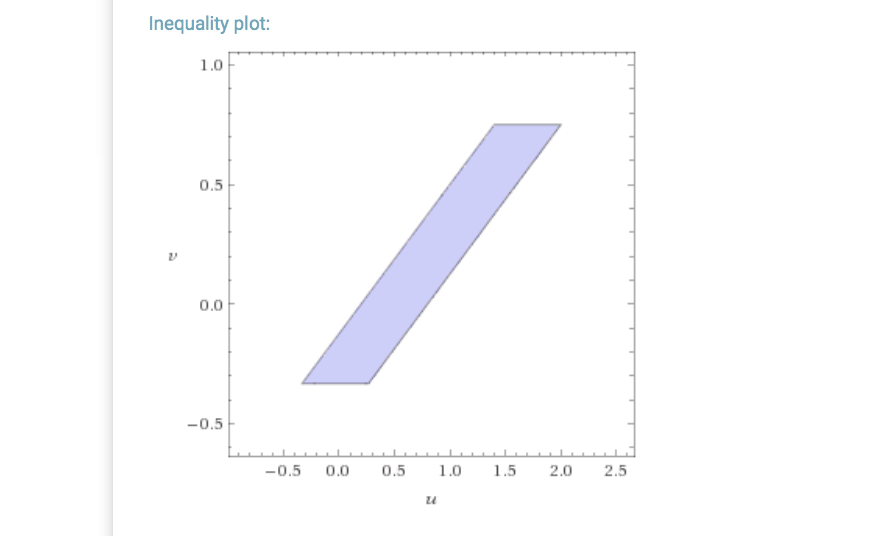
\includegraphics[width = 60mm, height=40mm]{images/7.png}
	\end{center}
	\begin{gather*}
	\begin{cases}
	-1 \leqslant y \leqslant 1 \\[2pt]
	-4 + 2y \leqslant 3x \leqslant -1 + 2y 
	\end{cases}
	\end{gather*}
	\begin{center}
		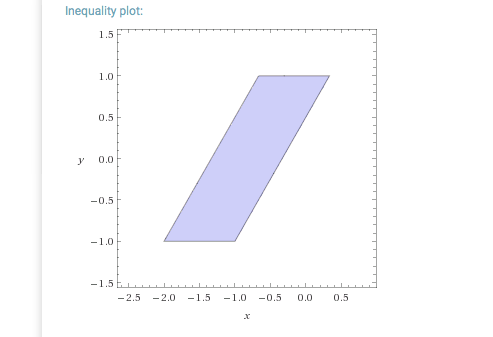
\includegraphics[width = 60mm, height=40mm]{images/8.png}
	\end{center}
\newpage



\textbf{\large Задача 22}
\medskip\hrule\medskip
\textit{Найдите и изобразите множество точек.(28)}
\begin{gather*}
\begin{cases}
x > -2 \\[2pt]
y > 1 \\[2pt]
2x + y < 1
\end{cases}
\begin{cases}
x = u - 2v \\[2pt]
y = u^2 + v^2
\end{cases}
\end{gather*}
Подставим в нашу систему $ x $ и $ y $:
\begin{gather*}
\begin{cases}
u - 2v > -2 \text{ - прямая }\\[2pt] 
u^2 + v^2 > 1 \text{ - внешняя окружность с центром $ (0, 0)  $   и радиусом 1}\\[2pt]
2u - 4v + u^2 + v^2 = (u + 1)^2 + (v - 2)^2 - 5  < 1 \text{ - окружность  с центром $ (-1, 2) $ и радиусом $ \sqrt{6} $ }
\end{cases}
\end{gather*}
\begin{center}
	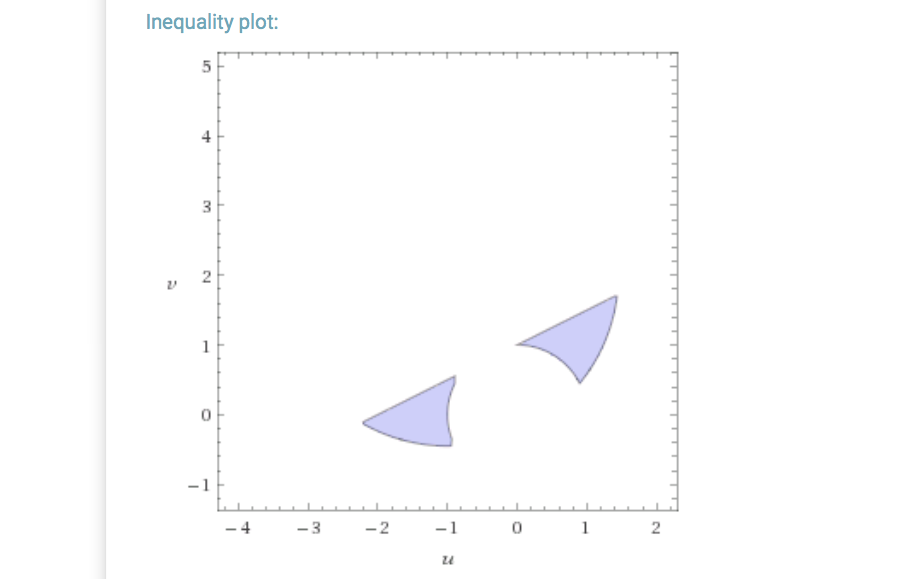
\includegraphics[width = 150mm, height=80mm]{images/9.png}
\end{center}










\end{document}